A carrier at frequency $f_c$ modulated by system activity is a lot easier to recognize if we generate periodic processor and/or memory activity that repeats $f_{alt}$ times per second. We will used the SAVAT micro-benchmarks (which create measurable periodic signals at arbitrary frequencies as described in Chapter~\ref{sec:savat}) to find AM modulated signals in computer systems. A modified version of one such micro-benchmark is shown in Figure~\ref{fase_pseudocode}. Recall that the loop beginning on line \ref{BegLoopA_fase} performs one activity (activity A), and the loop beginning on line~\ref{BegLoopB_fase} performs another activity (activity B). The outer loop repeatedly alternates activities A and B, creating periodically changing activity whose period equals the execution time for one iteration of the outer loop. This alternation period $T_{alt}$ is the inverse of the frequency $f_{alt} = \frac{1}{T_{alt}}$. Note that in Chapter~\ref{sec:savat}, we used this alternation to \emph{generate a carrier signal} at some chosen frequency $f_c$, while in this chapter we use this alternation at $f_{alt}$ to measure AM-modulation of any potential \emph{carrier signals intrinsically generated} (and emanated) by the system.

\begin{figure}[htb]
\lstset{language=C++,basicstyle=\ttfamily\footnotesize,numbers=left}\lstset{escapeinside={/*@}{@*/}}
\begin{lstlisting}[frame=none,xleftmargin=30pt]
while(true){/*@\label{BegInfLoop_fase}@*/
  // Execute the A activity /*@\label{BegLoopA_fase}@*/
  for(i=0;i<inst_a_count;i++){
    ptr1=(ptr1&~mask1)|((ptr1+offset)&mask1);/*@\label{UpdAddrA_fase}@*/
    // The A-instruction, e.g. a load from L2
    value=*ptr1;/*@\label{TestInstA_fase}@*/
  }/*@\label{EndLoopA_fase}@*/
  // Execute the B activity /*@\label{BegLoopB_fase}@*/
  for(i=0;i<inst_b_count;i++){
    ptr2=(ptr2&~mask2)|((ptr2+offset)&mask2);/*@\label{UpdAddrB_fase}@*/
    // The B-instruction, e.g a store from L2
    *ptr2=value;/*@\label{TestInstB_fase}@*/
  }/*@\label{EndLoopB_fase}@*/
}
\end{lstlisting}
\caption{Pseudo-code to generate the A/B alternation activity.}
\label{fase_pseudocode}
\end{figure}


As an example of how the alternation of activity can AM-modulate a carrier signal, consider a DRAM memory clock signal as shown in Figure~\ref{fig:alt_freq}. Activity A may involve many LLC misses, so it results in substantial DRAM activity. During the A-activity half-period, the DRAM clock drives a lot of switching activity (current flowing through wires), resulting in strong emanations at the DRAM clock frequency. If activity B has little DRAM activity, less switching activity is driven by the DRAM clock, generating weaker emanations at the DRAM clock frequency. Therefore the amplitude of the emanations at the DRAM clock frequency will change with period $T_{alt}$ (frequency $f_{alt}$), which means that emanations at the DRAM clock frequency will be AM-modulated by the A/B periodic behavior whose frequency is $f_{alt}$.

\begin{figure}[tbh]
  \centering
  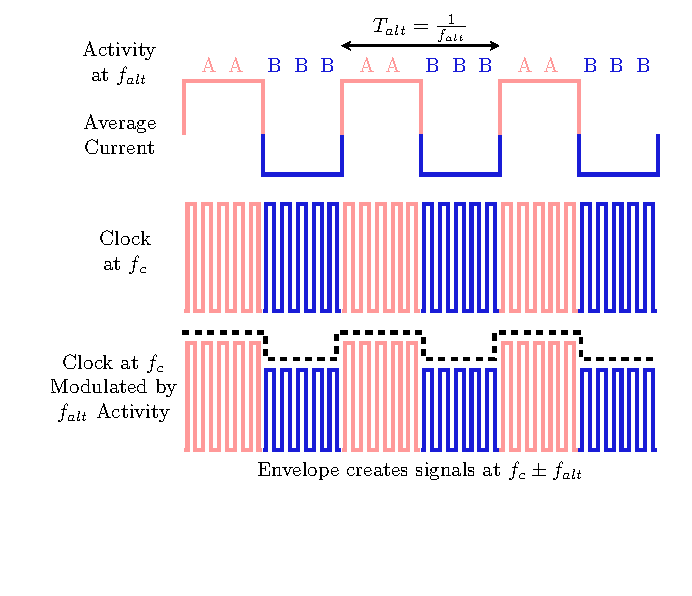
\includegraphics[width=5in]{../fase/Drawing/alt_freq.pdf}
  \caption{The micro-benchmarks do each of activities A and activity B for half the alternation period, resulting in a periodic component at the alternation frequency $f_{alt}$.}
  \label{fig:alt_freq}
\end{figure}

The key difference between the code shown in Figure~\ref{fase_pseudocode} and the SAVAT benchmarks described in Chapter~\ref{sec:savat} is that while the instruction counts for the A and B instructions were equal for SAVAT, for FASE we adjust the \texttt{inst\_a\_count} and \texttt{inst\_b\_count} variables so that activity A and activity B are each done for half of the alternation period (50\% duty cycle). Thus the spectrum of each side-band around the carrier's frequency $f_c$ will also have strong odd-numbered harmonics of the alternation frequency, i.e. the side-band signal will have spikes/peaks at $f_c \pm 3f_{alt}$, $f_c \pm 5f_{alt}$, etc. in addition to $f_c \pm f_{alt}$. Also note that the alternation frequency $f_{alt}$ can be controlled by changing the instruction counts, allowing us to create several separate spectra with sideband signals at different $f_{alt}$ frequencies. These spectra can be considered jointly in an effort to distinguish which carriers are modulated by a particular activity.

Finally, we use loads from memory (LDM), loads from the L2 cache (LDL2), and loads from the L1 cache (LDL1) as the activities A and B in the experiments we report. We have performed additional experiments with other activities (various arithmetic instructions) and have found that for the systems tested such activities modulate the same carriers that on-chip cache accesses do, so we use cache accesses as representatives of on-chip activity. Varying only the memory accesses in our code also allows us to eliminate all other code in the alternation loop as a possible source of modulation -- the address computation for all three types of memory accesses only differs in the values of the \texttt{mask1} and \texttt{mask2} parameters and the memory access instruction itself is also identical in all three cases.

FASE results for different A/B pairings usually provide a strong indication of which aspect of the system modulates a given carrier signal. For example, when a signal at a particular frequency $f_c$ is modulated by A/B alternation between memory activity and any on-chip activity, but remains unmodulated when alternating between two types of on-chip activity, the carrier signal and/or its modulation mechanism are likely related to the memory controller, processor-memory communication, or the DRAM memory itself.

As indicated in Section~\ref{sec:fase-am-devices}, discovery of activity-modulated carriers by ``eyeballing'' the spectrum without generating controlled system activity would be very difficult. Theoretically, one could look for narrow spikes (potential carriers) with symmetric side-bands on either side as shown in Figure~\ref{am_details_b}, but this approach is not practical due to the non-ideal nature of unintentional carriers, the interference of other signals, and noise as shown in Figure~\ref{am_details_e}.

\begin{figure*}[tb]
  \centering
    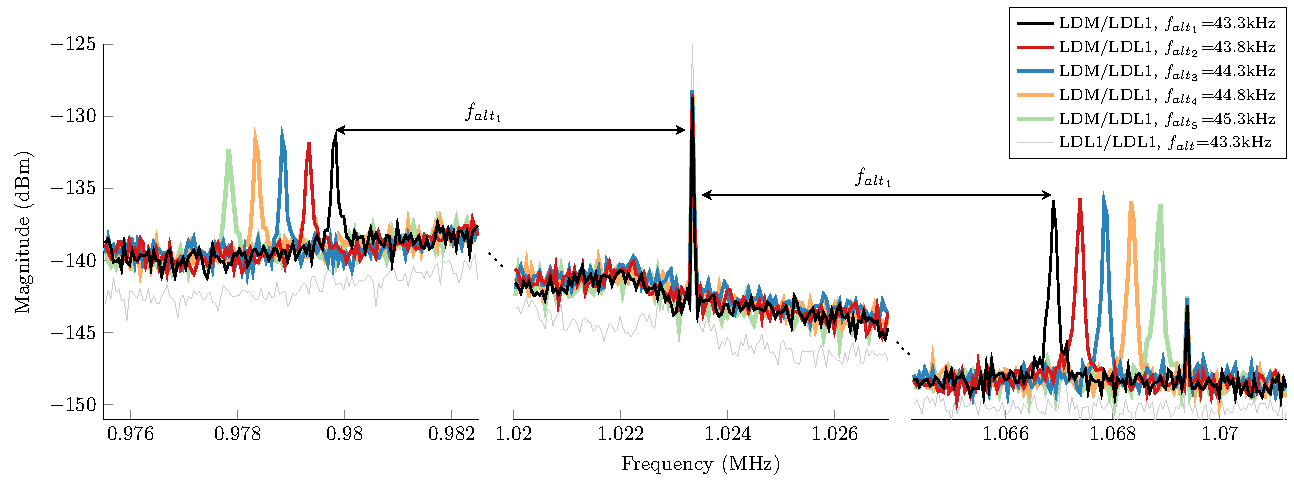
\includegraphics[width=\textwidth]{../fase/Data/mem_refresh_zoom.pdf}
  \caption{A carrier at $f_c$ and its right and left side-bands generated by memory activity.}
  \label{mem_refresh_zoom}
\end{figure*}

Measuring arbitrary programs or benchmarks may provide some information about carriers that are modulated by system activity but it would be difficult to determine the spectral properties of such arbitrary system activity. Even if we are somehow given spectral information about activity in an application, it would be hard to recognize whether the side-band signals around each potential carrier match that spectrum with high confidence because 1) amplitude modulation combines (convolves) the spectrum of the possibly non-ideal carrier signal with the arbitrary benchmark spectrum (Figure~\ref{am_details_d}), and 2) recognition of such a complicated overall spectrum is further hampered by noise and unrelated signals that overlap with portions of the modulated-signal spectrum (Figure~\ref{am_details_e}).
%
We cannot directly control the shape of a system's intrinsic carrier signals, but we can use SAVAT to generate system activity that is as close to a perfect square wave as possible. This results in side-band signals whose spectrum has a shape that closely matches the shape of the carrier signal they are modulating, with a $f_{alt}$ separation between the carrier and its two side-bands in the spectrum. This could be used to find carriers automatically by looking for such right and left side-band signals because they always appear as peaks in the spectrum separated by $2f_{alt}$ with the carrier peak half-way between them. However, this simplistic approach has a number of drawbacks. First, the alternation activity is a square wave which has many odd-numbered harmonics ($f_c \pm f_{alt}$, $f_c \pm 3f_{alt}$, etc.) that are separated by exactly $2f_{alt}$. This makes it difficult to attribute the spikes in the side-band signals to particular carrier frequencies, creating many false positive indications of carrier locations. Second, for some values of $f_{alt}$, some of the side-band signals may be overwhelmed by noise and unrelated signals, which would result in many false negatives. Third, computer systems contain many components with periodic activity, so unmodulated signals are often concentrated at specific frequencies. Some such spectral peaks will be nearly $2f_{alt}$ apart by random chance, resulting in more false positives.

Many of the problems caused by the harmonics of the alternation signal and by the existence of unrelated signals can be solved by performing multiple measurements with different alternation frequencies, e.g. $f_{alt_1}$, $f_{alt_2}=f_{alt_1}+f_\Delta$, $f_{alt_3}=f_{alt_1}+2f_\Delta$, etc., where $f_\Delta$ is typically small compared to $f_{alt}$. Figure~\ref{ideal_fase} illustrates an idealized diagram of the $f_{alt_N}$ side-bands with five such alternation frequencies. Figure~\ref{mem_refresh_zoom} shows five real spectra spectra with $f_{alt_1} = $ 43.3kHz and $f_\Delta = $ 0.5kHz around a carrier signal at $f_c =$ 1.0235MHz. To avoid clutter, Figure~\ref{mem_refresh_zoom} only shows the three parts of the spectrum that contain the left side-bands, the carrier, and the right side-bands of the signals. In other words, it does not show about 40kHz worth of spectrum to the left and right of the carrier. Note how the peaks in the side-bands move by $f_\Delta$ as the alternation frequency $f_{alt}$ changes by $f_\Delta$.

\begin{figure}[tbh]
  \centering
    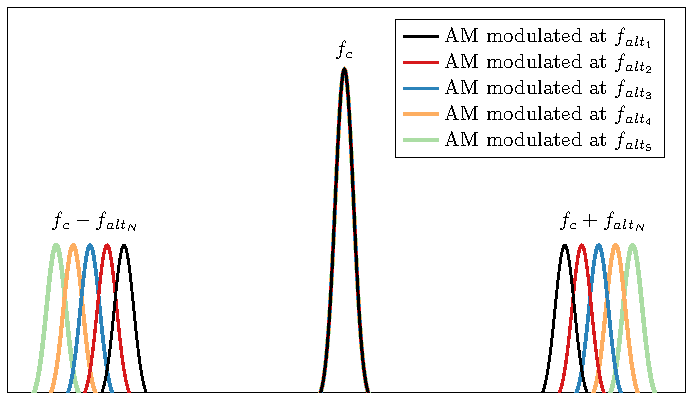
\includegraphics[width=\textwidth]{../fase/Data/ideal_fase.pdf}
  \caption{Ideal FASE spectral pattern illustrating an AM carrier at $f_c$.}
  \label{ideal_fase}
\end{figure}

Conceptually, the FASE methodology for finding activity-modulated carriers and determining the frequencies of such carriers is now as follows. First, perform several measurements (we use five) with different $f_{alt}$ frequencies as described above. Second, look for a shape in the spectrum that moves by $f_\Delta$ or $-f_\Delta$ in successive measurements. This approach eliminates external signals and system-emanated periodic signals that do not correspond to activity-induced AM modulation because such signals stay at the same frequency as $f_{alt}$ changes. It also only detects the first harmonic of $f_{alt}$ to the right and left of the carrier. Recall that the alternation activity changes abruptly and may not have a perfect 50\% duty cycle, so the spectrum of the modulated signal has side-band signals not only at $f_c \pm f_{alt}$ but also at $f_c \pm 2f_{alt}$, $f_c \pm 3f_{alt}$, etc. However, only the first harmonic ($f_c \pm f_{alt}$) moves by $f_\Delta$ in the spectrum as we change $f_{alt}$ by $f_\Delta$. The other harmonics in the side-band move by $2f_\Delta$, $3f_\Delta$, etc.

Once we have identified a first harmonic side-band signal in this way, we can determine whether it is the left side-band (moves by $-f_\Delta$) or the right one (moves by $f_\Delta$), and we can compute the frequency of its carrier signal. The carrier is located at $f - f_{alt_i}$ if the modulated peaks are detected at frequency $f$ and if $f_{alt_1}$ is to the left of $f_{alt_5}$ (or at $f+f_{alt_i}$ if $f_{alt_1}$ is to the right of $f_{alt_5}$). Note that detection of a single harmonic of $f_{alt}$ in a single side-band is sufficient to detect a carrier frequency, i.e. we do not need all of them to find the frequency of the carrier. Also, note that any harmonic (e.g. $\pm$2nd, $\pm$3rd, etc.) is sufficient since the observed spacing between the side-band peaks is unique for each harmonic (e.g. $2h_\Delta$ for the positive 2nd harmonic, -$3h_\Delta$ for the negative third harmonic, etc.). This comes in handy if one or more of the signals overlap with other signals or unusually strong noise -- with five measurements we get a total of ten side-band signals (two side-bands per measurement) at different frequencies, so we can reliably detect the presence of modulation and the frequency of the carrier even if several of the side-band signals are obscured as shown in the left side-band of Figure~\ref{core_reg_zoom}. Also note that this approach does not rely on actually observing a peak for the carrier signal. This is important when the carrier itself is located in a crowded part of the spectrum -- as long as at least a few side-band signals ``land'' in a ``quiet'' part of the spectrum, we can deduce the exact frequency of the carrier.

There often are several modulated carrier signals in the same general region of the spectrum, so that their side-band signals may not be neatly separated from each other. A simplified representation of one actual recorded spectrum is shown in Figure~\ref{core_reg_ldl2_harm}. The thick lines in this figure indicate carrier frequencies, each with a different color. The thin lines indicate the frequencies of side-band $f_{alt}$ harmonic signals, where the color indicates which carrier generates this side-band signal and the number indicates which harmonic of $f_{alt}$ it corresponds to. Without FASE the interleaved side-band signals generated by different carriers make it very difficult to manually interpret such measured spectra.

%\begin{comment} %--------------------
\begin{figure}[t]
  \centering
    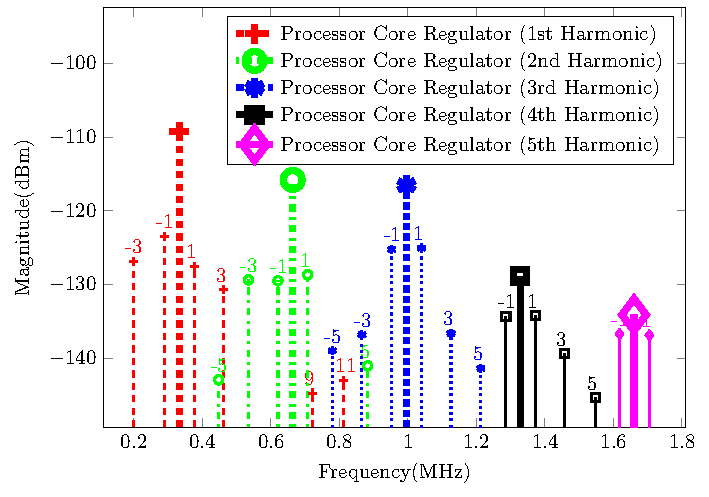
\includegraphics[width=5in]{../fase/Data/core_reg_ldl2_harm.pdf}
  \caption{Simplified spectrum representation of the harmonics of the LDL2/LDL1 activity for the Intel Core i7 desktop.}
  \label{core_reg_ldl2_harm}
\end{figure}
%\end{comment} %--------------------

The antennae we used to capture signals from computer systems were designed to detect broadcast radio signals over a wide frequency range, so they pick up these interfering signals very well. It is critical to note that FASE is intended to identify only AM signals which are modulated \textit{by our micro-benchmark}. Although AM radio signals are amplitude-modulated and strong, FASE correctly identifies that these signals are \emph{not caused by our modulation activity} and so should not be reported. This is important not only because it is painfully expensive to shield a measurement setup from broadcast signals, but also because computer systems themselves emit strong radio signals (wifi, bluetooth, NFC, etc.) that are modulated for communication purposes but should not be reported by FASE unless they are \emph{also} modulated by our microbenchmark activity.



